\chapter[Introdução]{Introdução}

Espaço reservado para Introdução.

\section{Contexto}
 
Espaço reservado para Contexto.

\section{Justificativa}

Espaço reservado para Justificativa.

\begin{table}[h!]
\centering
\begin{tabular}{|l|l|}
\hline
\textbf{Exemplo} & \textbf{Exemplo Tabela} \\ \hline
Teste1        & Exemplo1                         \\ \hline
Teste2         & Exemplo2                     \\ \hline
Teste3         & Exemplo3                        \\ \hline
Teste4            & Exemplo4                  \\ \hline
Teste5       & Exemplo5                   \\ \hline
\end{tabular}
\caption{Exemplo de Tabela.}\label{isquemia_orgaos}
\end{table}

\section{Escopo do projeto}
 \subsection{Premissas}
  
  Espaço reservado para Premissas.

  \subsection{Restrições}
  
  Espaço reservado para Restrições.

\section{Detalhamento do escopo}
 
 Espaço reservado para Detalhamento do escopo.

\section{Objetivos}

\subsection{Objetivo Geral}

Espaço reservado para Objetivo Geral.

\subsection{Objetivos Específicos}

Espaço reservado para Objetivos Específicos.

\section{Metodologia de gerenciamento}

Espaço reservado para Metodologia de gerenciamento.

\subsection{Plano de gerenciamento de comunicação}

Espaço reservado para Plano de gerenciamento de comunicação.

\subsubsection{Organização das reuniões}

Espaço reservado para agendamento organização das reuniões.

\subsubsection{Monitoramento e Controle}


Espaço reservado para Monitoramento e Controle.

\subsection{Plano de gerenciamento de riscos}

Espaço reservado para Plano de gerenciamento de riscos.


\subsection{EAP}

Espaço reservado para EAP.

\begin{figure}[H]
	\centering
%	\includegraphics[width=16cm]{figuras/eap.eps}
%	\caption{EAP - estrutura analítica do projeto} \label{eap}
\end{figure}

\subsection{Cronograma}

Espaço reservado para o cronograma.

\begin{figure}[H]
	\centering
%	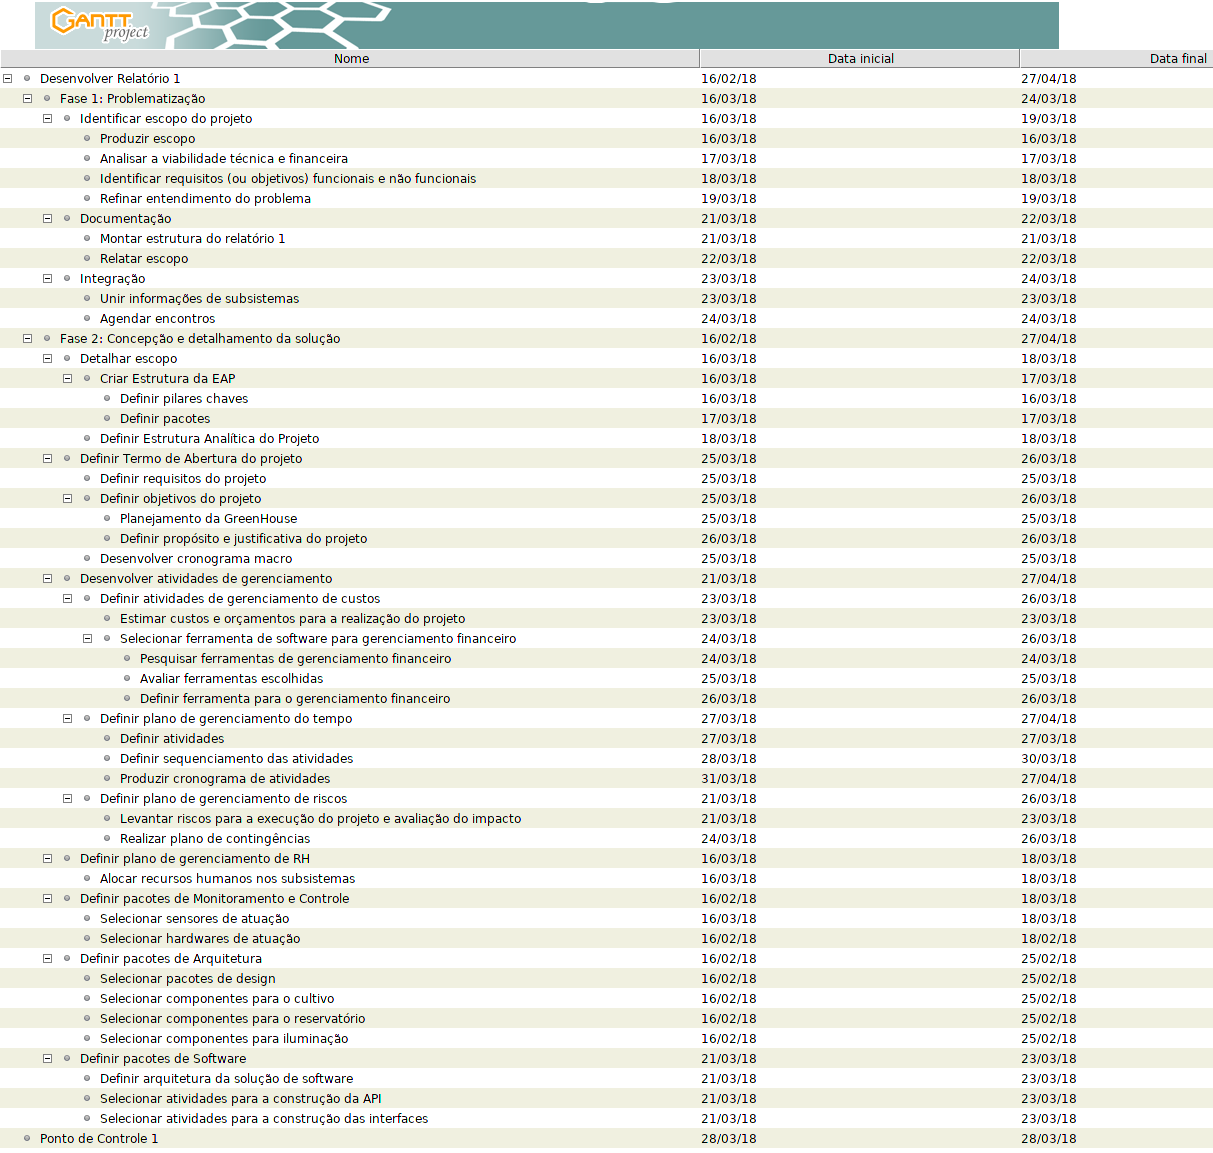
\includegraphics[width=16cm]{figuras/cronograma_1.eps}
	\caption{Cronograma do projeto} \label{cronograma_1}
\end{figure}

\begin{figure}[H]
	\centering
%	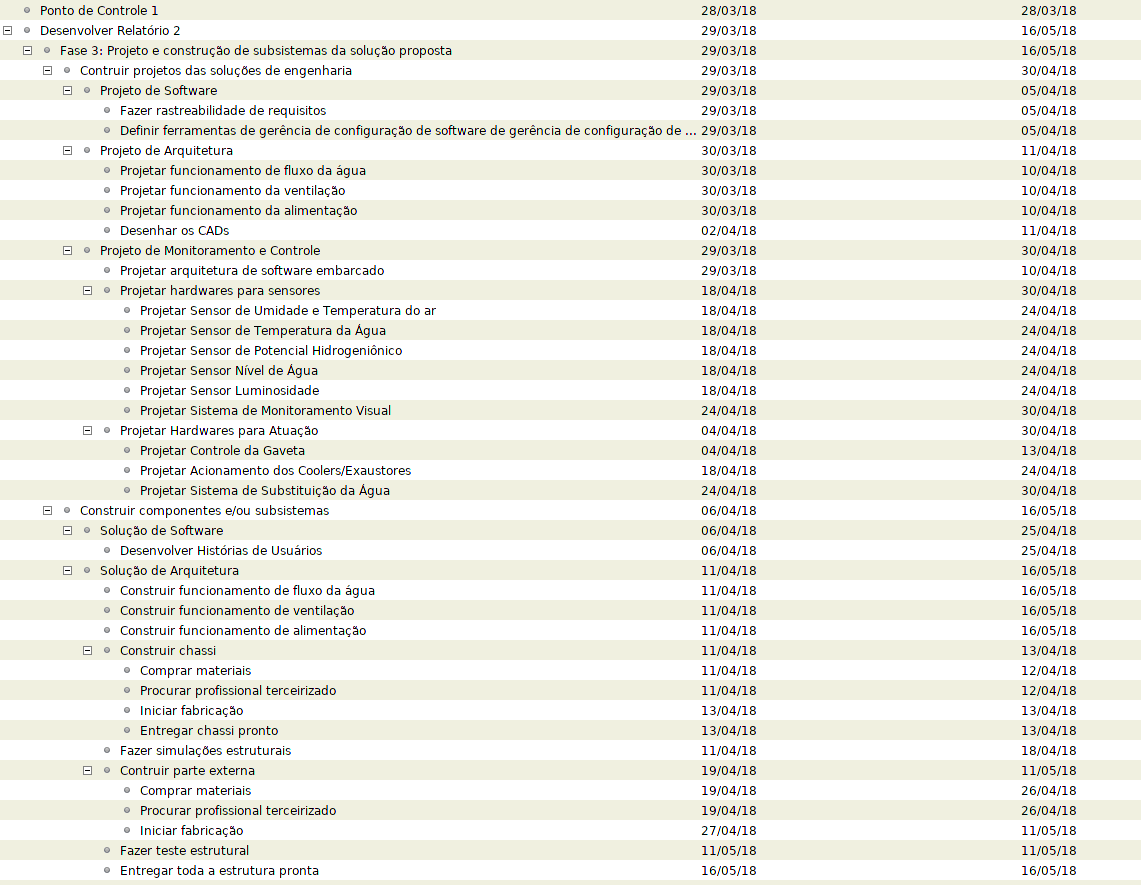
\includegraphics[width=16cm]{figuras/cronograma_2.eps}
	\caption{Cronograma do projeto} \label{cronograma_2}
\end{figure}




